% Nejprve uvedeme tridu dokumentu s volbami
\documentclass[slovak,master,dept460,male,cpp,cpdeclaration]{diploma}
% Dalsi doplnujici baliky maker
\usepackage[autostyle=true,czech=quotes]{csquotes} % korektni sazba uvozovek, podpora pro balik biblatex
%\usepackage[backend=biber, style=iso-numeric, alldates=iso]{biblatex} % bibliografie
\usepackage{dcolumn} % sloupce tabulky s ciselnymi hodnotami
\usepackage{subfig} % makra pro "podobrazky" a "podtabulky"
\usepackage{verbatim}
\usepackage{cite}
\usepackage{float}
\usepackage{amsfonts}
\usepackage{url}
\bibliographystyle{unsrt}
\nocite{*}
% Zadame pozadovane vstupy pro generovani titulnich stran.
\ThesisAuthor{Michal Falát}

\CzechThesisTitle{Analýza řidiče za pomocí sférických kamer}

\EnglishThesisTitle{Driver Analysis Using Spherical Cameras}

\SubmissionDate{1. apríla 2020}

% Pokud nechceme nikomu dekovat makro zapoznamkujeme.
\Thanks{Rád by som poďakoval môjmu vedúcemu práce Ing. Radovanovi Fusekovi za pomoc a ochotu pri vypracovaní diplomovej práce}

% Zadame cestu a jmeno souboru ci nekolika souboru s digitalizovanou podobou zadani prace.
% Pokud toto makro zapoznamkujeme sazi se stranka s upozornenim.
\ThesisAssignmentImagePath{Figures/Assignment1.jpg}
% \SlovakBachelorMaleAuthorDeclaration

% Zadame soubor s digitalizovanou podobou prohlaseni autora zaverecne prace.
% Pokud toto makro zapoznamkujeme sazi se cisty text prohlaseni.ss
% \AuthorDeclarationImageFile{Figures/AuthorDeclaration.jpg}


% Zadame soubor s digitalizovanou podobou souhlasu spolupracujici prav. nebo fyz. osoby.
% Pokud toto makro zapoznamkujeme sazi se cisty text souhlasu.
% \CooperatingPersonsDeclarationImageFile{Figures/CoopPersonDeclaration.jpg}

\CzechAbstract{Hlavnou témou diplomovej práce je rozpoznávanie a analýza vodiča v aute pomocou sférických kamier. Táto práca je rozdelená do viacerých samostatných častí. Prvá časť spočíva v samotnej detekcii ľudí a ich aktivít sférickou kamerou, hľadanie nedostatkov a nájdenie optimálnych parametrov pre čo najefektívnejšiu detekciu. Druhá časť je zameraná na porovnanie jednotlivych knižníc a metód, ktoré sa používaju na analýzu ľudského tela a tváre v obraze. Posledná časť je venovaná porovnaniu týchto metód s použitím reálnych dát zachytených sférickou kamerou a zhrnutie výsledkov. }

\CzechKeywords{Sférická kamera, detekcia obrazu, analýza ľudskej tváre, detekcia ľudí, vodič}

\EnglishAbstract{Main focus of this Diploma thesis is detection and analysis of driver in car with help of spherical cameras. This thesis is divided into few parts. The first part is about detection itself, detection of people by spherical cameras, research of disadvantages and finding optimal parameters for most efficnet detection. The second aprt is focused on comparision of libraries used for  human body and face detections. The last part is  about comparision of libraries with  real datas captured by  spherical camera and summary of results.  }

\EnglishKeywords{Spherical camera, image detection, analysis of human face, pedestrian detection, driver }


\AddAcronym{2D}{2-dimensional}
\AddAcronym{3D}{3-dimensional}
\AddAcronym{CNN}{Convolutional neural network}
\AddAcronym{CPU}{Central processing unit}
\AddAcronym{FPS}{Frames per second}
\AddAcronym{GPU}{Graphical processing unit}
\AddAcronym{HOG}{Histogram oriented gradients}
\AddAcronym{IR} {Infra red}
\AddAcronym{LED} {Light emitting diode}
\AddAcronym{NMS} {Non maximum suppression}
\AddAcronym{OpenCV} {Open source computer vision}
\AddAcronym{PAF}{Part afinity fields}
\AddAcronym{PX}{Pixel}
\AddAcronym{RCNN}{Region convolutional neural network} 
\AddAcronym{SPPE}{Single-person pose estimator}
\AddAcronym{SSTN}{Symmetric spatial transformer network}
\AddAcronym{TF}{Tensorflow}
\AddAcronym{VR}{Virtual reality}



% Novy druh tabulkoveho sloupce, ve kterem jsou cisla zarovnana podle desetinne carkyss
\newcolumntype{d}[1]{D{,}{,}{#1}}


% Zacatek dokumentu
\begin{document}

% Nechame vysazet titulni strany.
\MakeTitlePages

% A nasleduje text zaverecne prace.
\section{Úvod}
\label{sec:Introduction}
V dnešnom modernom svete sú autá takmer každodennou súčasťou života ľudí. Mnohokrát sa ani nezamýšľame nad ich bezpečnosťou, ktorá je v prípade zrážky kľúčová. V súčasnosti nám pri jazde autom asistuje veľké množstvo systémov, ktoré zvyšujú bezpečnosť posádky, ale aj ostantých účastníkov cestnej premávky. Aj keď tieto systémy ešte stále nedokážu vodiča úplne nahradiť, dokážu mu výrazným spôsobom pomôcť napríklad v krízových situáciach. Výhodou takýchto systémov je ich rýchlejší reakčný čas oproti človeku. Takéto systémy spočívajú v použití rôznych snímačov alebo kamier, ktoré aktívne sledujú okolie ale aj interiér vozidla. Vďaka takýmto moderným technickým riešeniam je možné predísť rôznym  častokrát aj smrteľným dopravným nehodám. Výrobcovia áut sa čoraz častejšie snažia svoje systémy vylepšovať na čo najvyššiu možnú úroveň a poskytnúť tak vysoký level ochrany.\par Táto diplomová práca sa zameriava hlavne na problematiku analýzy vodiča pomocou detekcie obrazu zo sférickej (360-stupňovej) kamery. V diplomovej práci som sa venoval analýze videa z kamery umiestnenej v interiéri vozidla. Vhodným umiestnením kamery je možné získať obraz zpred auta, ale aj obraz vodiča sediaceho za volantom. V tejto práci som sa zameriaval na analýzu a spracovanie videa z interiéru vozidla na zachytenie ľudských aktivít vodiča. Aby som získal čo najväčšiu časť tela vodiča, je potrebné mať dostatočne veľký uhol záberu. Bežné kamery majú uhol záberu veľmi nízky, aby dokázal z malej vzdialenosti zachytiť celý snímaný objekt. Takýto problém sa naskytuje najpríklad aj v interiéri vozidla, kde je vzdialenoť kamery od snímaného objektu menej ako 1 meter, čo nemusí byť dostatočné na zosnímanie tela celého vodiča. Práve v takejto situácii je vhodné použiť širokouhlú prípadne sférickú kameru. Počas práce som mal k dispozicii viaceré kamery, s ktorými som zhotovol niekoľko desiatok videí v rôznych situáciach. Z takýchto videi som dokázal analyzovať a zistiť mnoho užitočných informácii, ktore sú spracované v tejto diplomovej práci. Tieto informácie som zbieral nahrávaním videa sférickymi kamerami za rôznych svetelnych  podmienok a pozicií vodiča. V tejto práci sú taktiež spomenuté problémy takejto analýzy, riešenia vzniknutých problémov, ale aj zhrnutie celkovej problematiky sledovania vodiča vo vozidle. V práci sú tiež zhrnuté ďalšie možnosti vylepšenia detekcie a porovnanie oproti klasickým kamerám.\par V nasledujúcich kapitolách je postupne rozobratá problematika snímania ľudských postáv v obrazoch, a skúmanie ich aktivít. Pre snímanie postavy som sa rozhodol použiť viacero metód, ktoré som následne porovnal a zanalyzoval. Aby som vedel vyhodnotiť správnu pozíciu vodiča, rozhodo lso msa  použiť neurónovú sieť, ktorú som trénoval na vlastnom datasete.\par V súčasnosti som taktiež nenašiel veľa riešení na spracovanie videa zo sférickej kamery a preto by som sa snažil zamerať túto prácu hlavne na túto oblasť. Pri analýze vodiča som taktiež nenašiel vhodné datasety z interiéru vozidla snímané sférickou kamerou.




\newpage
\section{Detekcia a analýza ľudského tela v obrazoch}
\label{sec:human body decection}

História detekcie postáv v obrazoch siaha až do polovice 20. storočia.  Mnoho inžinierov videlo obrovský potenciál detekcie obrazu napríklad v oblastiach medicíny, priemyslu, dopravy a mnohých ďalších oblastiach. S nárastom technických možností postupne rástla aj motivácia využiť detekciu obrazu aj v praxi. Jeden z prvých vedeckých článkov v oblasti spracovania obrazu \cite{rosenfeld1969} rozoberal napríklad jednoduchú analýzu  obrazu a spracovanie obrazov s dostupnými prostriedkami.  Postupom času sa však počítačová technika vylepšovala a bolo možné pracovať na vývoji metód pre analýzu  a detekciu objektov v obrazoch. Na detekciu chodcov alebo iných ľubovolných objektov existuje mnoho prístupov. Veľkým fenoménom v posledných rokoch sa stali neurónové siete. Okrém neurónových sietí však stále existujú aj tradičné metódy, ktoré fungujú aj bez trénovacích dát. Vo svojej práci som pracoval hlavne s metódami Haar a HOG, ktoré sa radia medzi najpoužívanejšie tradičné metódy a sú im venované samostatné podkapitoly \ref{Haar} a \ref{HOG}.\par
Každý obraz sa skladá z pixelov. Analýza obrazu však nespočíva v prehľadávani jednodlivých pixelov, ale v hľadaní jednotlivých objektov v obraze. Tieto objekty je možné  určovať do  samostatných tried. Triedy nám určujú, aký druh objektu sa v obraze nachádza (Napríklad chodec, vozidlo, dopravná značka a podobne). Aby bolo možné tieto objekty (v našom prípade ľudí) nájsť, bolo potrebné nájsť spoľahlivý a rýchly spôsob detekcie. 


\subsection{Haar}
\label{Haar}
Táto metóda bola popísaná autormi Viola a Jones\cite{viola2001rapid} v roku 2001. Medzi jej hlavné výhody patrí vysoká rýchlosť  a spoľahlivá detekcia a vysoká nezávislosť na intenzite osvetlenia. Vo všeobecnosti je tento detektor rozdelený do 4 samostantných častí: Výpočet integrálneho obrazu,  výpočet Haar príznakov, výber príznakov a kaskádový klasifikátor.\par Výpočet integrálneho obrazu sa robí prevedením vstupného obrazu na integrálny obraz (Obr. \ref{fig:integralImage}). Výpočet pre konkrétne súradnice \textit{(x, y)} spočíva v súčte hodnôt jasu vľavo a nad súradnicami  \textit{(x, y)}. Výpočet je znároznený v rovnici \ref{eq:integral}.


\begin{figure}[H]
	\centering
	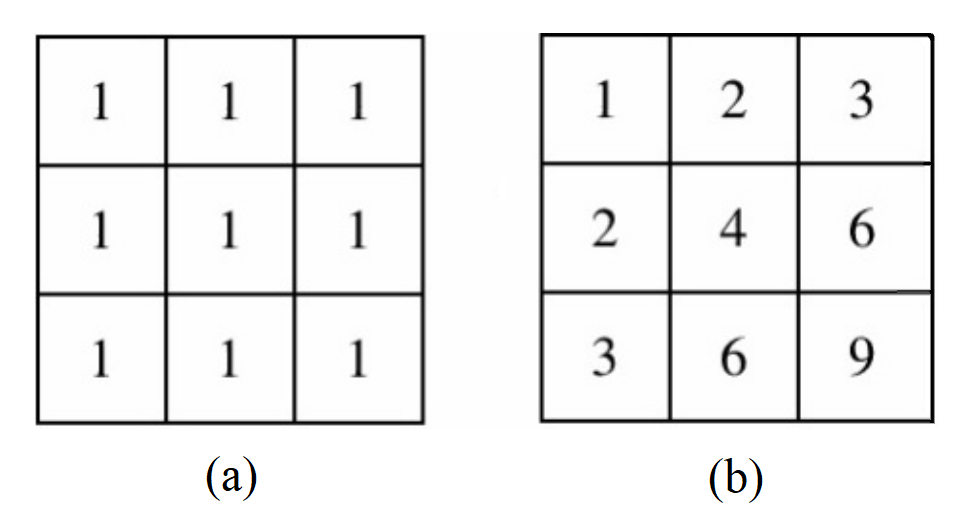
\includegraphics[width=0.5\textwidth]{Figures/integralImage.png}
	\caption{Výpočet integrálneho obrazu - vstupný obraz (A) , integrálny obraz (B)}
	\label{fig:integralImage}
\end{figure}


\begin{equation}
ii(x,y)=\sum_{x^{\prime}\leq x,y^{\prime}\leq y}i(x^{\prime},y^{\prime}),
\label{eq:integral}
\end{equation}


 Metóda funguje na porovnavaní celých blokov pixelov. Tieto bloky (častokrát nazývané aj zhluky) môžu mať rôzne tvary, veľkosť a natočenie. Tieto bloky môžu nadobúdať rôzne tvary ale vo všeobecnosti sa používajú 3 hlavné typy príznakov:
\begin{itemize}
  \item \textbf{Dvoj-obdĺžnikové} \textit{(angl. two-rectangle)} - porovnávajú sumu pixlov v obdĺžnikových oblastiach, ktoré sa nachádzajú vedľa seba, vodorovne, alebo zvislo.
  \item \textbf{Troj-obdĺžnikové} \textit{(angl. three-rectangle)} - porovnávajú sumu obdĺžnikových oblastí, ktoré sa nachádzajú po oboch stranách aktuálnej oblasti a sumu aktuálnej oblasti.
  \item \textbf{Štvor-obdĺžnikové} \textit{(angl. four-rectangle)} - počítajú rozdiel medzi dvoma aktuálnymi obdĺžnikovými oblasťami, ktoré sa dotýkajú svojimi rohmi, a obdĺžnikovými oblasťami medzi nimi.
  
 \end{itemize}
   \begin{figure}[H]
	\centering
	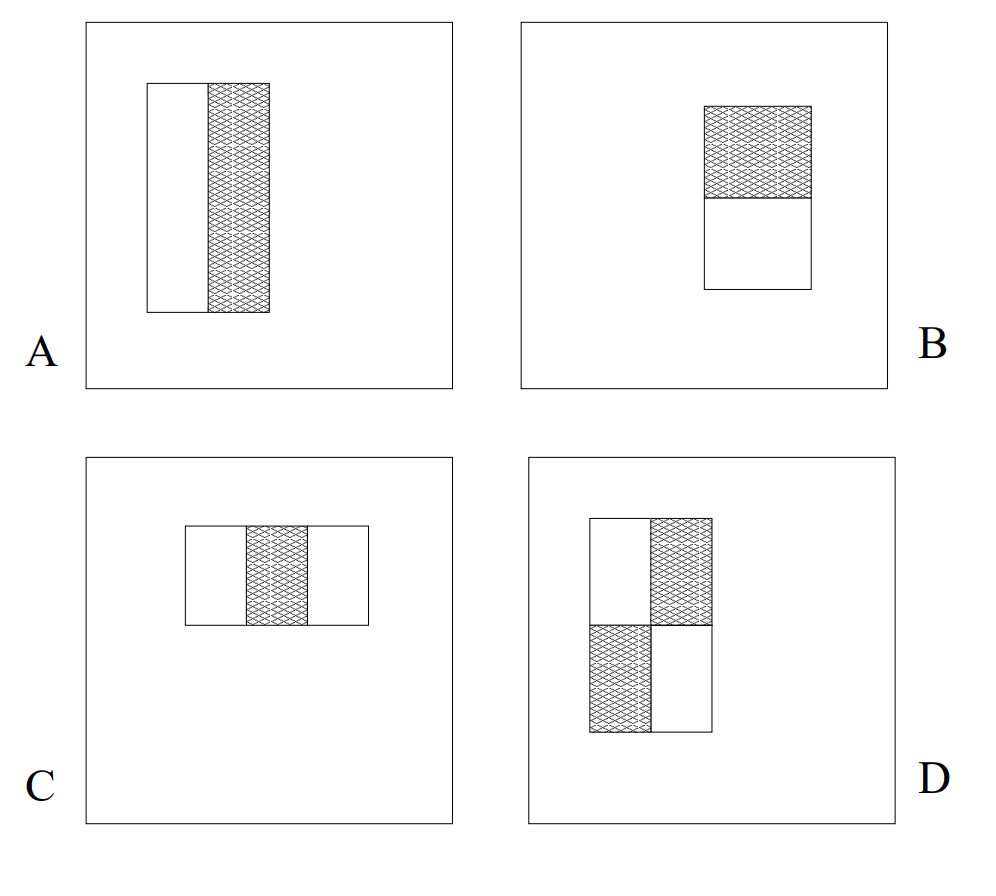
\includegraphics[width=0.6\textwidth]{Figures/haar1.png}
	\caption{Haar - dvoj-obdĺžnikové príznaky (A, B), troj-obdĺžnikové príznaky (C) a štvor-obdĺžnikové príznaky(D)\cite{viola2001robust}}
	\label{fig:Haar1}
\end{figure}
  Znázornenie jednotlivých typov príznakov môžeme vidieť na obrázku \ref{fig:Haar1}. Jednotlivé príznaky môžu byť použité dostatočne efektívne. Efektivita klesá pri použití príznaku na celý obraz. Vhodným riešením je preto skombinovať viacero príznakov. Na výber  správnych efektívnych príznakov sa používajú špeciálne algoritmy. Jedným z najpoužívanejších algoritmov  pre zvýšenie efektivity výberu príznakov je AdaBoost\cite{freund1995desicion}, ktorý vytvoril profesor Yoav Freund. Jedná se o klasifikačný algoritmus, ktorý je schopný vytvoriť dostatočne silný klasifikátor z kombinácii viacerých slabších klasifikátorov.  Metódou Haar je možné detekovať rôzne triedy objektov.  Jedným z najčastejších a jednoducho detekovatelných  typov objektov je napríklad tvár.


\begin{figure}[H]
	\centering
	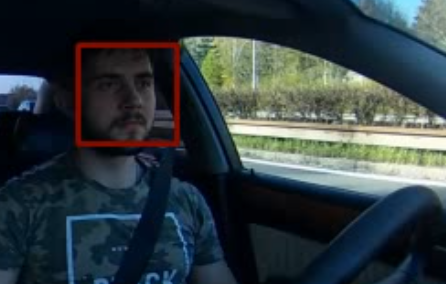
\includegraphics[width=0.6\textwidth]{Figures/haar2.png}
	\caption{Haar - detekcia tváre v slabých svetelných podmienkach}
	\label{fig:Haar2}
\end{figure}



\subsection{HOG}
\label{HOG}
S nápadom  vylepšiť detekciu objektov použitím príznakov prišli v roku 2005 Navneed Dalal a Bill Triggs \cite{dalal2005}, kde postupne vyskúšali niekoľko typov deskriptorov.  V práci taktiež podrobne rozobrali  možnosti a spôsoby ako správne určiť parametre ich detekčnej metódy pre správne fungovanie detekcie jednotlivých tried. Hlavnou myšlienkou ich metódy je, že objekt môže byť charakterizovaný  viacerými spôsobmi. Táto metóda je rozdelená do niekoľkých samostatných krokov (Obr. \ref{fig:HOG1}):
\begin{itemize}
  \item \textbf{Úprava obrazu} - v tomto kroku je potrebné  v obraze upraviť kontrast a jas , ktoré by mohli spôsobovať  problémy v nasledujúcich krokoch. Okrem tejto úpravy  je možné  obraz urpaviť napríklad gamma filtrom.
  \item \textbf{Výpočet gradientov} - veľkosť gradientov sa počíta na základe vstupného obrazu a masky. Masky, ktoré sa používaju v tomto kroku sú \textit{[-1, 0, 1]} alebo \textit{[-1, 0, 1] \textsuperscript{T}}. Gradienty je nutné vypočítať v obidvoch osách, čím získame \textit{I\textsubscript{x}} a \textit{I\textsubscript{y}}. Po získaní gradientov je potrebné vypočítať veľkosť gradientov \textit{m(x,y)} a ich smer \textit{$\theta(x, y)$}:
  
\begin{equation}
m(x,y)= \sqrt{I_{x}^{2} + I_{y}^{2}}
\label{eq:Výpočet veľkosti gradientu}
\end{equation}

  \begin{equation}
\theta(x, y) = \left(\frac{I_{y}}{I_{x}}\right)
\label{eq:Výpočet smeru gradientu}
\end{equation}
  \item \textbf{Normalizácia} -  Pre správne fungovanie je potrebné obraz normalizovať, aby sa minimalizovali rozdiely medzi jednotlivými bunkami. Tento krok spočíva v skladaní viacerých buniek, čím následne vznikajú bloky. 
   \item \textbf{Deskriptor} -  Je vytvorený zo vstupného obrazu do jednotlivých blokov. Jednotlivé bloky sa posúvajú a prekrývajú o daný počet pixelov. Výsledok desktiproru je odovzdaný  klasifikátoru, ktorý následne určuje do akej triedy objekt patrí. Jeden z často používaných klasifikátorov je Support vector machine (SVM), ktorý napríklad používali autori práce na efektívnu detekciu chodcov.\cite{pang2011efficient}
 \end{itemize}


\begin{figure}[H]
	\centering
	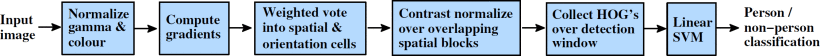
\includegraphics[width=1\textwidth]{Figures/hog.png}
	\caption{HOG - séria krokov \cite{dalal2005}}
	\label{fig:HOG1}
\end{figure}

Výstupom tejto metódy je pole histogramov pre jednotlivé bloky. Histogram predstavuje grafické rozloženie intenzity jasu vstupného obrazu. Pri niektorých špecifických obrazoch je potrebné histogram vyrovnať. Tento krok je potrebný najmä pri obrazoch, ktoré su príliš tmavé alebo príliš svetlé. Pomocou vyrovnania \textit{(angl. equalization)} histogramu  dokážeme zvýšiť kontrast obrazu. Jednotlivé kroky znázornené na vstupnom obraze chodca môžeme vidieť na obrázku \ref{fig:HOG2}\par


\begin{figure}[H]
	\centering
	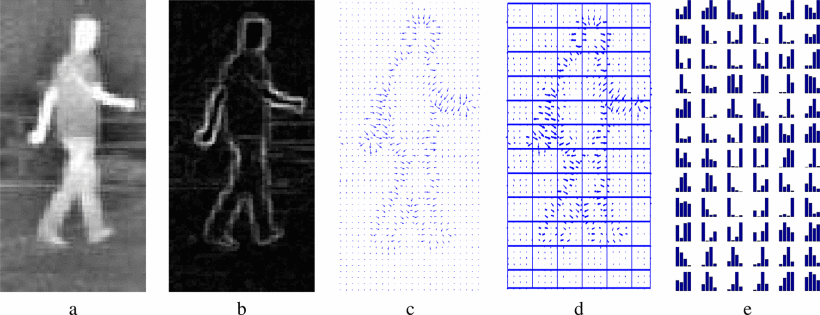
\includegraphics[width=1\textwidth]{Figures/hog3.png}
	\caption{HOG - vstupný obraz (a), normalizácia gradientu (b), orientácia gradientu (c), rozdelenie do buniek (d) vypočítané histogramy (e). \cite{bertozzi2007pedestrian}}
	\label{fig:HOG2}
\end{figure}


\newpage
\subsection{OpenPose}
OpenPose\cite{cao2018openpose} je framework, ktorý bol prvýkrat uvedený verejnosti už v roku 2016. Detekcia ľudského postoja predstavuje hlavný problém s lokalizáciou častí ľudského tela, ako sú ramená, lakte a členky zo vstupného obrázka alebo videa. Vo väčšine dnešných aplikácií detekcie postaáv v reálnom svete sa vyžaduje vysoký stupeň presnosti, ako aj spracovanie v reálnom čase.
OpenPose, ktorý bol vyvinutý výskumníkmi na univerzite Carnegie Mellon University, možno považovať za najmodernejší prístup pri detekcii ľudských v reálnom čase. Jedná sa o open-source projekt, ktorého zdrojové kôdy sú dostupné na oficiálnej Github stránke \cite{githubOpenpose}.

\begin{figure}[H]
	\centering
	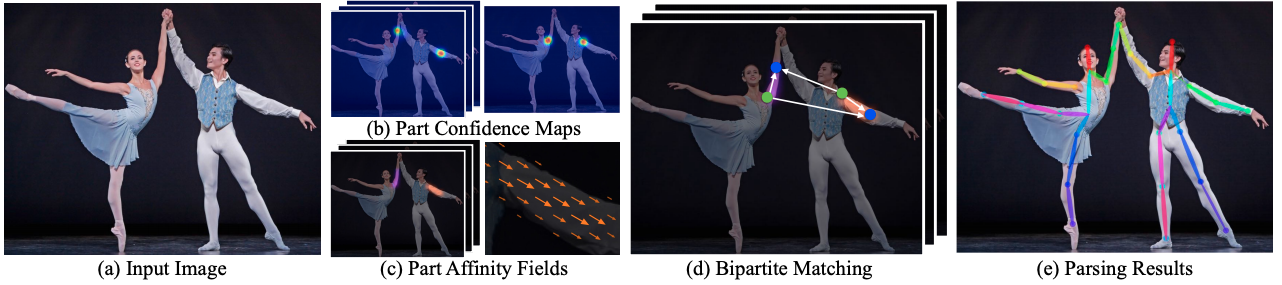
\includegraphics[width=1\textwidth]{Figures/openposePipeline.png}
	\caption{OpenPose - odhad viacerých ôsob v reálnom čase pomocou polí afinity filtra.\cite{cao2018openpose}}
	\label{fig:openposeOverall}
\end{figure}

 Samotný framework je veľmi detailne vysvetlený a dobre zdokumentovaný. OpenPose bol pôvodne napísaný v C++ a Caffe\cite{jia2014caffe}. Postupom času však  autori vytvorili aj  nadstavbu pre jazyk Python, s ktorým sa rozšírili možnosti jeho využitia medzi ostratnými programátormi. Základná myšlienka detekcie pomocou OpenPose sa skladá z viacerých krokov:

\begin{itemize}
\item \textbf{Spracovanie vstupného obrazu} - vstupný obrázok (Obr. \ref{fig:openposeOverall}a) privádza ako vstup do „dvojvetvového viacstupňového“ CNN. Dve vetvy znamenajú, že CNN produkuje dva rôzne výstupy z jedného vstupného obrazu. Viacstupňové jednoducho znamená, že sieť je v každej fáze naskladaná jedna na druhú. (Tento krok je analogický jednoduchému zväčšeniu hĺbky neurónovej siete s cieľom zachytiť podstatnejšie výstupy smerom k posledným stupňom.)

\item \textbf{Spracovanie v dvoch vetvách} - prvá vetva predpovedá mapy dôveryhodnosti (Obr. \ref{fig:openposeOverall}b) rôznych častí tela, ako je pravé oko, ľavé oko, pravé lakte a podobne. Druhá vetva zobrazená modrou farbou predpovedá afinitné polia (Obr. \ref{fig:openposeOverall}c), čo predstavuje stupeň asociácie medzi rôznymi časťami tela.

\item \textbf{Viacfázové spracovanie} - v prvej fáze sieť vytvorí počiatočnú sadu detekčných máp spoľahlivosti \textit{S} a množinu polí afinity častí \textit{L}. Potom v každej nasledujúcej fáze predpovede z obidvoch vetiev v predchádzajúcej fáze, spolu s pôvodnými obrazovými znakmi \textit{F}, sú zreťazené a použité na vytvorenie podrobnejších predpovedí. Pri implementácii OpenPose sa posledná fáza \textit{t} zvolí ako  číslo 6.
\end{itemize}

\subsubsection{Mapa spoľahlivosti}
1. vetva v neurónová sieti OpenPose vytvára sadu máp spoľahlivosti \textit{S} (rovnica \ref{eq:confidencemap}). V podstate sa jedná o tabuľku, v ktorej je každej časti tela z datasetu priradená miera spoľahlivosti v rozsahu 0 až 1. 

\begin{eqnarray}
& S = (S_{1}, S_{2}, S_{3} ... S_{j}) \label{eq:confidencemap}\\
& S\in\mathbb{R}^{w \times  h},\nonumber\\
& j\in \left \{1,\: J  \right \}, kde\: J\: je\: počet\: všetkých\: častí\: tela\nonumber
\end{eqnarray}
Počet častí tela závisí od množiny datasetov, s ktorými je program OpenPose trénovaný. Pokiaľ ide napríklad o súbor datasetu COCO\cite{lin2014microsoft}, \textit{J = 19}, pretože existuje 18 rôznych kľúčových bodov tela + 1 pozadie. Obrázok \ref{fig:cocoDataset} zobrazuje rôzne časti tela s prideleným ID pre súbor údajov COCO. Pre model trénovaný s dátovým súborom COCO bude sada \textit{S} obsahovať prvky \textit{S1, S2, S3,…, S19}. V tomto príklade predpokladáme, že prvok \textit{S1} zodpovedá mape spoľahlivosti pre kľúčový bod s číslom 0 ktorý zodpovedá nosu (Obr. \ref{fig:cocoDataset}).\par Pre ľahšiu predstavu predpokladáme, že celý obraz má šírku a výšku 5px, čo vedie k vytvoreniu  mapy spoľahlivosti o veľkosti \textit{$5\times 5$}. Vo vstupnom obrázku sa nachádza iba jedna tvár. Preto pre mapu spoľahlivosti \textit{S1} (zodpovedajúca za detekciu nosa) vidíme hodnoty s vysokou spoľahlivosťou iba v oblasti, kde sa nos nachádza.\bigskip

\begin{figure}[H]
	\centering
	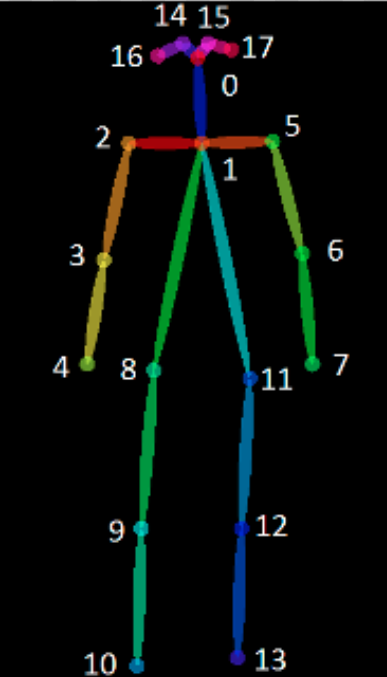
\includegraphics[width=0.3\textwidth]{Figures/cocoDataset.png}
	\caption{COCO - označenie častí tela v COCO datasete.\cite{cocoDataset}}
	\label{fig:cocoDataset}
\end{figure}


\subsubsection{Part afinity fields (PAF)}
Druhá vetva neurónovej siete vytvára množinu čiastkových afinitných polí \textit{L} (rovnica \ref{eq:pafmap}).

\begin{eqnarray}
& L = (L_{1}, L_{2}, L_{3} ... L_{c}) \label{eq:pafmap}\\
& L\in\mathbb{R}^{w \times  h \times 2},\nonumber\\
& c\in \left \{1,\: C  \right \}, kde\: C\: je\: počet\: všetkých\: končatín\nonumber
\end{eqnarray}

Celkový počet končatín a párov, závisí od datasetu, s ktorým je OpenPose trénovaný. Kvôli prehľadnosti sa uvádzajú dvojice častí tela ako končatiny, napriek tomu, že niektoré páry častí tela nie sú v skutočnosti končatinami (Napríklad oko-nos, ucho-oko atď). Pre dataset COCO je počet párov končatín, \textit{C = 19}. Môžeme si predstaviť, že každý prvok v množine \textit{L} je mapa veľkosti \textit{$w\times h$}, kde každá bunka obsahuje 2D vektor predstavujúci smer párových prvkov. Napríklad na obrázku \ref{fig:cocoDataset} môžeme vidieť, že pár častí tela pozostáva z pravého ramena k pravému laktu. Schéma potom ukazuje smerový vektor, ktorý ukazuje z pravého ramena na pravý lakeť. Celý zoznam párov končatín môžeme vidieť vo výpise \ref{src:coco_pairs}.\bigskip

\begin{lstlisting}[language=Python,label=src:coco_pairs,caption={Množina párov končatín v datasete COCO}]
COCO_PAIRS = [(1, 2), (1, 5), (2, 3), (3, 4), (5, 6), (6, 7), (1, 8), (8, 9), (9, 10), (1, 11), (11, 12), (12, 13), (1, 0), (0, 14), (14, 16), (0, 15), (15, 17), (2, 16), (5, 17)]
\end{lstlisting}

\bigskip
Okrem Datasetu COCO Dokáže OpenPose pracovať aj s mnohými ďalšími datasetmi. OpenPose bol skúšaný a trénovaný napríklad s datasetmi MPI, BODY\_25 alebo BODY\_25b. Datasety sa líšia vo veľkosti, rýchlosti, ale napríklad  aj v presnosti samotnej detekcie. Jednotlivé datasety majú medzi sebou nasledujúce rozdiely:


\begin{itemize}
\item \textbf{COCO} - je starší dataset, na ktorom bol OpenPose pôvodne vyvíjaný. Postupne sa však nahradzuje novými a modernejšími datasetmi. Jeho výhodou je, že vyžaduje menej pamäte na GPU (schopnosť pracovať s 2 GB GPU a predvoleným nastavením) a pri režíme CPU pracuje rýchlejšie oproti novšiemu BODY\_25.

\item \textbf{BODY\_25} - jedná sa o novší dataset, ktorý je rýchlejší, presnejší a obsahuje ďalšie trénovacie dáta k častiam tela, ktoré nie sú obsiahnuté v COCO datasete (Napr. chodidlá). Jeho nevýhodou sú hlavne vysoké hardwarové nároky.

\item \textbf{MPI} - je určený pre ľudí, ktorí požadujú štruktúru datasetu MPI. Je tiež pomalší oproti BODY\_25 a oveľa menej presný
\end{itemize}




\newpage
\subsection{TF Pose Estimation}
Tento framework pre detekciu postáv bol implementovaný pomocou knižnice Tensorflow. Poskytuje tiež niekoľko variantov, ktoré sa odlišujú najmä v zmenách pre spracovanie v reálnom čase na CPU alebo zariadení s nízkou spotrebou. Z tohto dôvodu je  možné používať napríklad na mobilných zariadeniach alebo internetových prehladiačoch použitím knižnice tensorflow.js. Tensrflow Pose estimation používa na detekciu  vlastný model s názvom PoseNet. PoseNet sa dá použiť na odhad jednej pozície alebo viacerých pozícií  v obraze súčasne. To znamená, že existuje verzia algoritmu, ktorý dokáže detekovať iba jednu osobu v obraze a druhá verzia, ktorá dokáže zistiť viac osôb v obraze. Hlavnou výhodou použitím detekcie jednej osoby je rýchlejšie spracovanie   a nižší výpočtový výkon. Podstatnou nevýhodou však je, že vyžaduje iba jeden objekt prítomný na obrázku. Pri súčasnej pozícii viacerých osôb v obraze tento algoritmus nedokáže zdetekovať správne ani jednu osobu. Je preto potrebné sa zamyslieť sa  hneď na začiatku, koľko ôsob sa reálne môže v obraze nachádzať. Hlavná myšlienka tohto algoritmu sa skladá z dvoch krokov podobne ako pri knižnici OpenPose.

\begin{itemize}
\item \textbf{Detekcia pozície} - na najvyššej úrovni modelu PoseNet sa vráti objekt, ktorá obsahuje zoznam kľúčových bodov a skóre spoľahlivosti pre každú detekovanú osobu.
\item \textbf{Výpočet spoľahlivosti pozície} - skóre spoľahlivosti určuje celkovú dôveru v odhadovaní pozície. Je v rozsahu od 0 až 1. Môže sa použiť na skrytie pozícií, ktoré sa nepovažujú za dostatočne výrazné.
\item \textbf{Výpočet kľúčových bodov} - odhadované časti tela osoby, ako napríklad nos, pravé ucho, ľavé koleno, pravá noha atď. Obsahuje pozíciu a spoľahlivosť kľúčového bodu. PoseNet štandardne zisťuje 17 kľúčových bodov.
\item \textbf{Poloha kľúčového bodu} - pozostáva z 2D súradníc  v pôvodnom vstupnom obrázku, kde bol zistený kľúčový bod.
\end{itemize}


Model PoseNet je nezávislý na veľkosti vstupného obrazu. To znamená, že môže predikovať polohy pozícií v rovnakom rozlíšení ako pôvodný obrázok bez ohľadu na to, či je obraz zmenšený. PoseNet môže byť nakonfigurovaný tak, aby mal vyššiu presnosť na úkor rýchlosti detekcie nastavením výstupného kroku. Výstupný krok určuje, do akej miery zmenšujeme výstup vzhľadom na veľkosť vstupného obrázka. To ovplyvňuje veľkosť jednotlivých vrstiev a výstupy modelu. Čím vyšší je výstupný krok, tým menší je počet vrstiev v sieti a výstupoch a tým aj ich presnosť. V základnej implementácii môže mať výstupný krok hodnoty 8, 16 alebo 32. Inými slovami, výstupný krok 32 bude mať za následok najrýchlejší výkon, ale najnižšiu presnosť, zatiaľ čo 8 bude mať najvyššiu presnosť, ale najpomalší čas detekcie.


\subsubsection{Výstup}
Keď PoseNet spracováva obraz, v skutočnosti vytvára tepelnú mapa \textit{(angl. Heatmap)} spolu s ofsetovými vektormi, ktoré je možné dekódovať, aby sa v obraze našli oblasti s vysokou spoľahlivosťou. Veľkou výhodou pri detekcii postáv v obraze cez Tensorflow je teda to, že spolu s vektormi výstupného modelu dostávame aj štruktorované dáta pravdepodobnosti jednotlivých častí postavy, ktoré môžeme využiť na ďalšie spracovanie, alebo znázorniť\textit{(Obr. \ref{fig:tfPoseHeatmap})}.

\subsubsection{Tepelná mapa}
Každá pozícia v tejto tepelnej mape má určité skóre spoľahlivosti. Tento údaj vyjadruje pravdepodobnosť, že v danom umiestnení existuje určitá časť daného typu. Dá sa to považovať za rozdelenie pôvodného obrázka do mriežky \textit{$15\times 15$}, kde skóre v termografickej mape poskytuje klasifikáciu pravdepodobnosti, že každý kľúčový bod existuje v každom štvorci mriežky.

\subsubsection{Výstupný vektor}
Každý ofsetový vektor je 3D vektor, ktorý má veľkosť \textit{$Šírka obrazu \times výška obrazu \times 34$}. Číslo 34 je dvojnásobok kľúčových bodov( 2 * 17). Tepelné mapy sú iba aproximáciou toho, kde sa skutočné kľúčové body nachádzajú, pričom výstupné vektory zodpovedajú svojou polohou bodom tepelnej mapy a používajú sa na predpovedanie presnej polohy jednotlivých častí ľudského tela. Prvých 17 rezov výstupného vektora obsahuje x-ovú súradnicu vektora a posledných 17 rezov y-ovú súradnicu. Veľkosti výstupného vektora sú v rovnakej mierke ako pôvodný vstupný obrázok.

\begin{figure}[H]
	\centering
	\includegraphics[width=1\textwidth]{Figures/tfPose1.png}
	\caption{Tepelná mapa  - vstupný obraz (a), tepelná mapa postavy (b)}
	\label{fig:tfPoseHeatmap}
\end{figure}

\subsection{AlphaPose}
AlphaPose\cite{fang2017rmpe} je framework, ktorý vznikol v roku 2017. Je zameraný na detekciu ľudských postáv  v čo najpresnejšej miere. Tento framework pracuje na princípe používania ohraničovacích boxov \textit{(angl. bounding box)}. Pre efektívne fungovanie algoritmu je použitý najmodernejší detektor objektov. Autori práce použili natrénovaný model Faster RCNN\cite{ren2015faster} a model pre detekciu postáv v obraze\cite{newell2016stacked}, ktorý je zameraný na SPPE detekciu. Primárna myšlienka práce spočíva v riešení dvoch hlavných problémov, ktoré pri takejto detekcii vznikajú:
\begin{itemize}
\item \textbf{Problém lokalizačnej chyby} - skutočnosti je SPPE dosť náchylný na chyby pri spočívajúce v použití ohraničovacích boxov. Aj v prípadoch, keď sú ohraničovacie rámčeky
sú považované za správne a majú dostatočne vysokú spoľahlivosť \textit{$(I_oU > 0,5)$}, zistené ľudské pozície môžu byť stále nesprávne. 
\item \textbf{Redundantná detekcia} - SPPE vytvára pózu pre každý ohraničovací box, čo vo výsledku vedie k duplicitnej detekcii rovnakej osoby (Obr.\ref{fig:alphaPoseRedundant})
\end{itemize}

\begin{figure}[H]
	\centering
	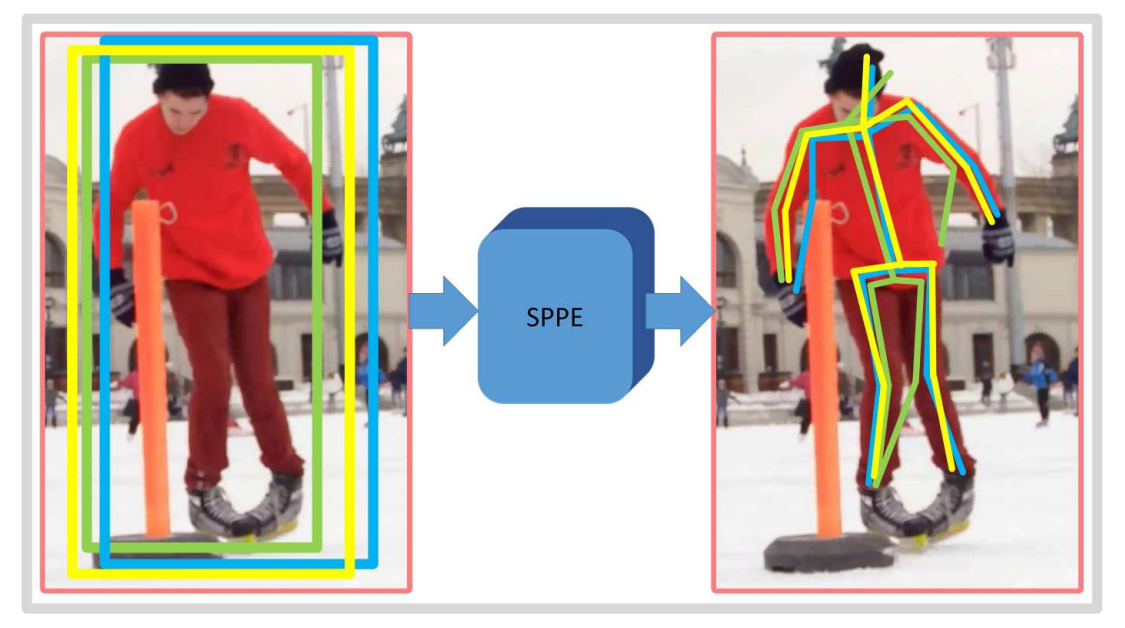
\includegraphics[width=0.6\textwidth]{Figures/alphaPoseRedundant.png}
	\caption{Problém redundantnej detekcie s použitím metódy bounding box\cite{fang2017rmpe}}
	\label{fig:alphaPoseRedundant}
\end{figure}

Na vyriešenie uvedených problémov je použitý model na regionálnu detekciu viacerých postáv (RMPE). Vďaka tomu
framework vylepšuje výkon algoritmov na odhadovanie ľudských postojov založených na SPPE. Autori práce tiež navrhli novú
symetrickú sieť pre priestorovú detekciu (SSTN), ktorá je pripojená k SPPE na extrakciu jednotlivej osoby z
oblasti nepresného ohraničovacieho boxu. Na optimalizáciu tejto siete je zavedená ďalšia paralelná vetva SPPE. Na riešenie problému redundantnej detekcie, je použitý parametrický NMS, ktorý eliminuje nadbytočné pózy pomocou novej metriky vzdialenosti a porovnanie podobnosti pózy. Prístup založený na údajoch je
aplikovaný na optimalizáciu parametrov metriky vzdialenosti. RMPE je navrhnutý veľmi všeobecne a práve vďaka tomu je použiteľný pre rôzne ľudské detektory a ďalšie knižnice, ktoré pracujú na princípe single-person detection. AlphaPose používa dataset MPII , s ktorým prekonáva najmodernejšie metódy ako OpenPose. Tento model a zdrojové kódy\cite{githubAlphaPose} sú verejne dostupné a určené primárne pre vedu a výskum.

\newpage
\subsection{Ostatné metódy}
Okrem  najpoužívajenších metód ako OpenPose a TF pose estiamtion, či AlphaPose existuje aj mnoho ďalších riešení. Tieto riešenia často vychádzajú zo základného princípu detekcie postáv, ktoré používajú aj tieto hlavné knižnice. Hlavný rozdiel je však použitie upravenej neurónovej siete alebo zmena rôznych parametrov. Vďaka takejto úprave je možné dosiahnúť v špecifických prípadoch vyššiu úspešnosť a presnosť detekcie alebo dokonca znížiť výpočtový čas potrebný na detekciu a spracovanie. Tieto riešenia sú však často obmedzované najmä chýbajúcou dokumentáciou , nedostatočnou implementáciou vo viacerých jazykoch, alebo nemožnosťou jednoduchej zmeny konfigurácie. Okrem voľne dostupných riešení existuje aj mnoho projektov, ktoré nie sú OpenSource, čo môže mnoho používateľov zo začiatku odradiť. V nasledujúcom odseku sú zhrnuté a v krátkosti rozpísané ďalšie knižnice, ktoré sa používajú na detekciu postáv v obrazoch.



\subsubsection{WrnchAI}
WrnchAI je framwork, ktorý bol vytvorený už v roku 2014. S myšlienkou využiť umelú inteligenciou a založiť projekt pre detekciu postáv prišiel Paul Kruszewski. Napriek tomu, že tento framework  existuje už niekoľko rokov a v niektorých článkoch\cite{openposeVsWrnchAI} dokázal dokonca získať lepší čas detekcie oproti iným metódam,  nestal sa natoľko populárnym medzi vývojarmi. Jedným z hlavných dôvodov je to, že knižnica nie je voľne dostupná pre vývojárov a jedná sa o platený projekt bez voľného prístupu k zdrojovému kódu. Súčasná cenová politika základnej verzie sa pohybuje na úrovni \$500 za mesiac používania s možnosťou vyskúšania trial verzie na 1. mesiac zadarmo. Trial verzia však funguje v obmedzenom režime  bez prístupu ku všetkým platformám. Pre bežného človeka sa táto cena môže zdať privysoká, avšak vzhľadom na jeho široké možnosti využitia  v rôznych oblastiach sa jedná o adekvátnu cenu. WrnchAI však našiel svoje uplatnenie možnosťou využitia na rôznych typoch zariadení, ktoré sa prispôsobujú konkrétnym podmienkam. V súčasnosti WrnchAI poskytuje 4 hlavné platformy:
\begin{itemize}
\item \textbf{wrnchPC} - umožňuje zachytiť ľudský pohyb od toľkých ľudí, koľko chcete, bez toho, aby ste museli nosiť ťažkopádne senzory. Náš tretí AI motor je agnostický fotoaparát, hardvérový AI hardvér, vyrobený tak, aby sa ľahko integroval do všetkých aplikácií. Používame spoľahlivé modely hlbokého učenia, aby sme zabezpečili spoľahlivé zachytenie ľudského pohybu pre všetky činnosti a v akomkoľvek prostredí


\item \textbf{wrnchCloud} - detekuje ľudský postoj a pohyb z akéhokoľvek video vstupu. WrnchCloud je nákladovo veľmi efektívne riešenie, pretože nepotreje žiadne vysoké hardwarové nároky okrem bežného počítača s pripojením na internet. Celý proces detekcie prebieha na serveri, čo odbremenuje zákaznika od nákupu drahých grafických kariet a podobne. Toto riešenie je škálovateľné s možnosťou spracovania viacerých vstupov súčasne. Využitie cloudového riešenie zároveň pomáha držať krok moderných trendov v internetových technológiách.

\item \textbf{wrnchMobile } - umožňuje využiť mobilné zariadenia na vytvorenie programu snímania postáv v reálnom čase. Taktiež dokáže spolupracovať s mobilnými operačnými systémami ako Android alebo IOS. Jeho základnym princípom je efektívne využitie výpočtového výkonu  na malých prenosných zariadeniách ako sú napríklad mobilné telefóny. Tento druh platformy taktiež dokáže pracovať aj s dalšími pokročilými vecami ako je napríklad rozšírená realita. S touto pomocou rozšírenej reality dokáže wrnchMobile snímanú postavu detekovať a zároveň zobrazovať napríklad do VR okuliarov.


\item \textbf{wrnchEmbedded} - poskytuje možnosť detekovať postavy na rôznych automatizovaných zariadeniach ako napríklad roboty,  samoriadiace vozidlá, aby mohli v reálnom čase vidieť a interagovať s ľuďmi a ich pohybom. WrnchEmbedded pomáha zariadeniam predvídať ľudské správanie a najlepšie reagovať vo všetkých situáciách. Ich program je optimalizovaný najmä na rôzne priemyselné platformy a počítače, vďaka ktorým by mala byť ich integrácia s platformou Wrnch veľmi jednoduchá. V Súčasnsnoti je však táto časť platformy stále v aktívnom vývoji a nie je dostupná. 
\end{itemize}

\begin{figure}[H]
	\centering
	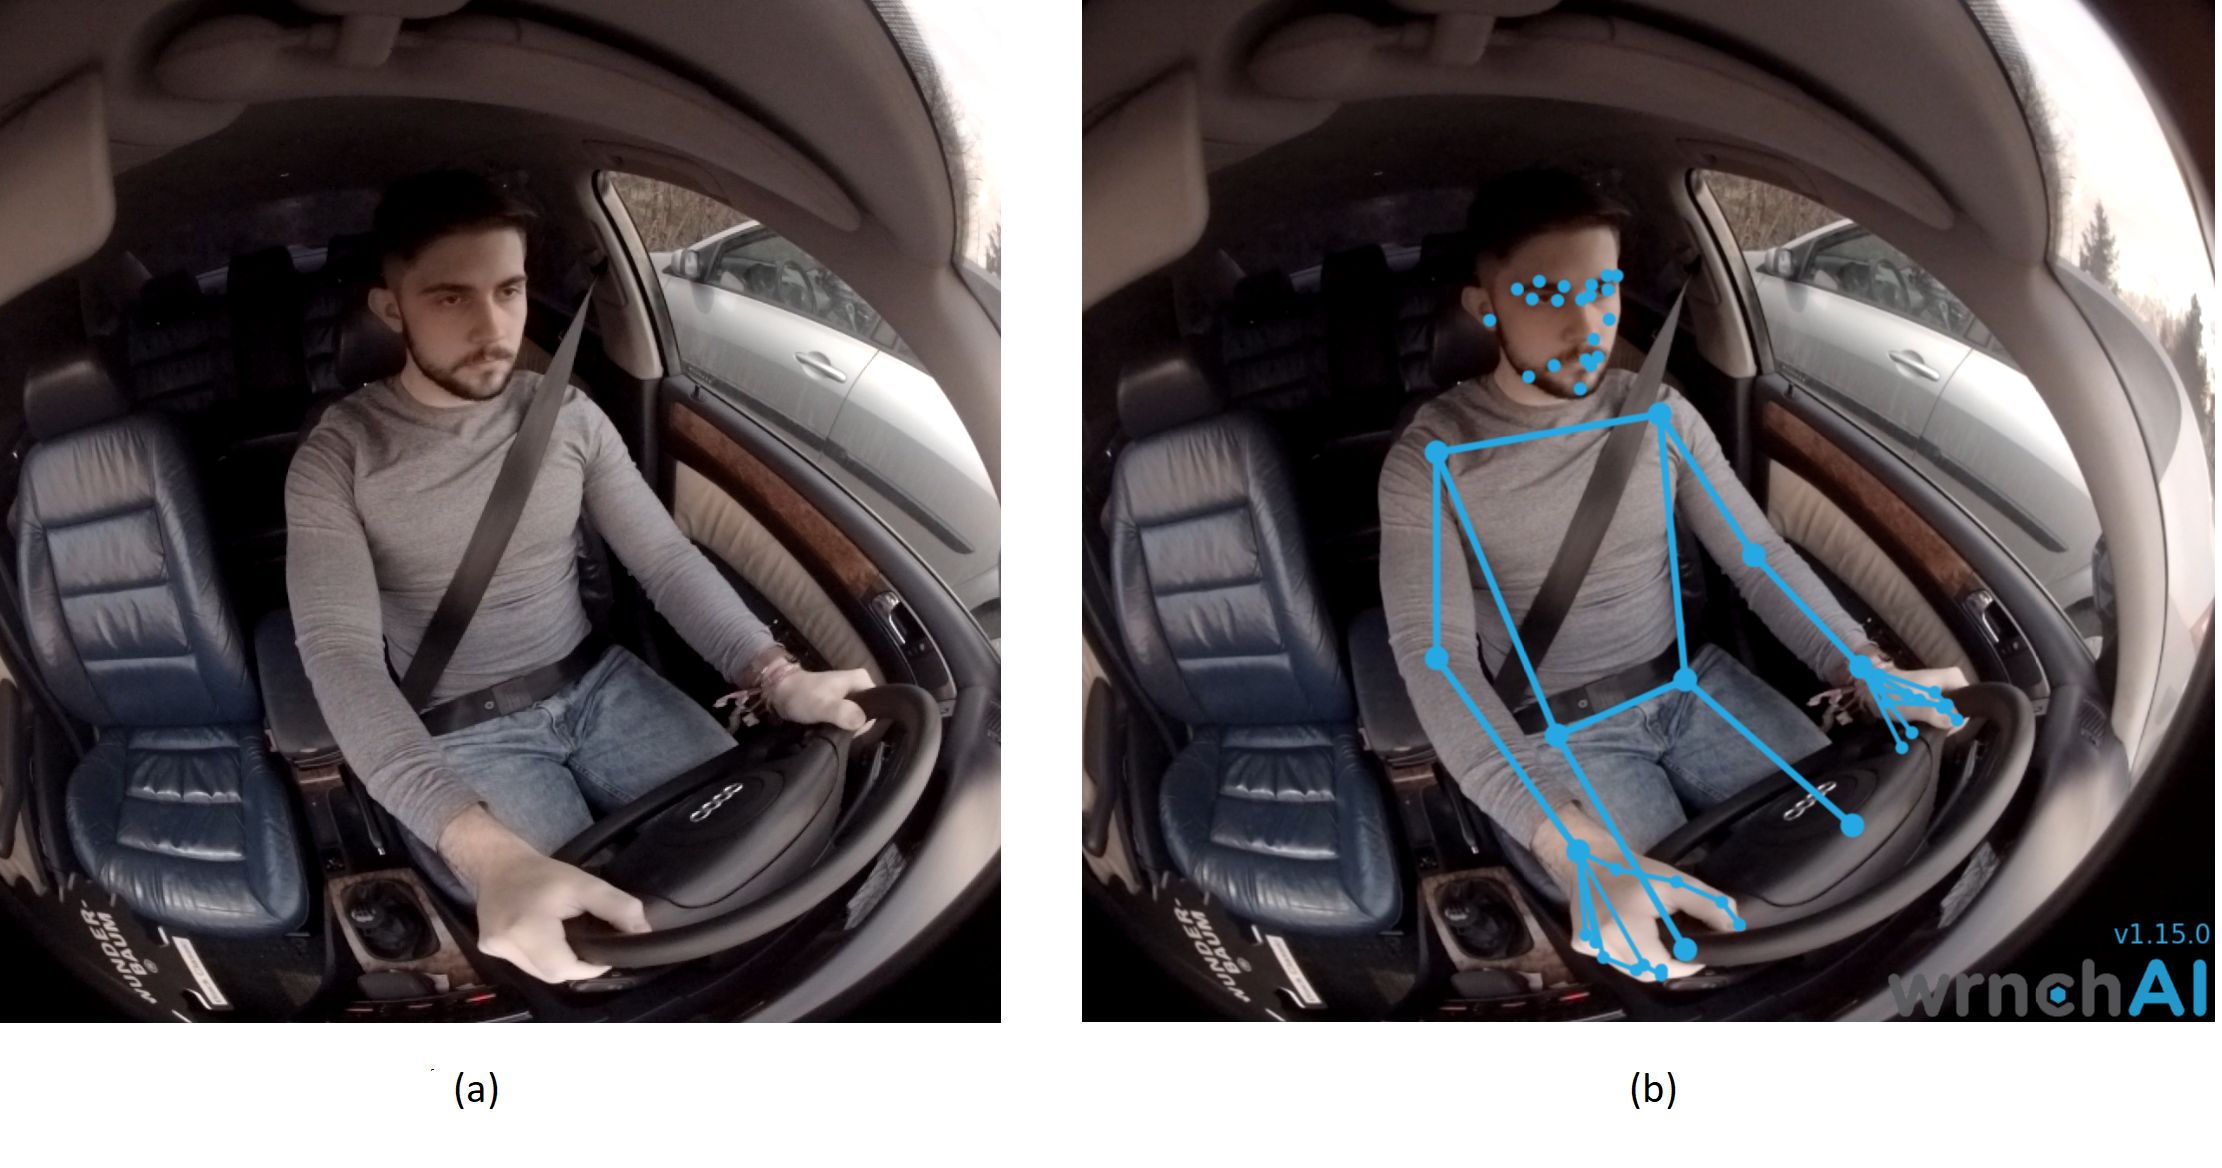
\includegraphics[width=1\textwidth]{Figures/wrnchAI.png}
	\caption{WrnchAI - vstupný obraz (a), výsledok spracovania na platforme WrnchAICloud(b)}
	\label{fig:wrnchAICloud}
\end{figure}

Na obrázku \ref{fig:wrnchAICloud} môžeme vidieť výsledok metódy cloudovej platformy WrnchAI. Táto platforma  funguje dostatočne spoľahlivo aj aj pri atypických polohách ľudského tela, ako je napríklad sedavá poloha vodiča za volantom. WrnchAI okrem polohy tela poskytuje aj detekciu kľúčových bodov tváre a kľúčové body rúk a prstov. Oproti ostatným knižniciam a frameworkom je možnost použiť WrnchAI ako komplexne riešenie na detekciu celého ľudského tela, čo napríklad pri OpenPose nieje bez použitia dalších rozšírené možné. V skúšobnej trial verzii  taktiež nieje možné odstrániť vodoznak firmy, ktorý sa nachádzav pravom dolnom rohu výstupného obrázka.


\newpage
\section{Detekcia vodiča vo vozidle}
\label{sec:Pose detection}
Detekcia objektov v uzavretom priestore (v našom prípade vo vozidle) sa od bežnej detekcie v základných princípoch nelíši. Obmedzenia nastávaju najmä nevhodnou pozíciou alebo natočením kamery. Ak je kamera nesprávne umiestnená, alebo má nedostatočný uhol záberu, nemusí byť zdetekovaný celý snímaný objekt, čo môže viesť k chybe pri jeho detekcii. Autori v práci \cite{smith2003determining}, kde sa zameriavali na oblasť tváre vodiča použili kameru umiestnenú v oblasti stredu palubnej dosky. Tým dosiahli takmer priame natočenie kamery na vodiča , bez toho, aby ho táto kamera výraznejšie obmedzovala vo výhľade. Keďže táto práca bola zameraná primárne na detekciu očí a úst, nebolo potrebné  používať kameru s vysokým uhlom záberu. Mnoho podobných riešení zameraných na snímanie aktivity vodiča sa snažia zaviesť aj výrobcovia automobilov. Príkladom môže byť vyrobca  automobilov značky BMW, ktorý v príplatkovej výbave ponúka kameru na snímanie správania vodiča. Táto kamera dokáže reagovať napríklad na únavu alebo zatvorenie očí vodiča. Vo všeobecnosti tento systém dokáže dokonca reagovať aj na to, že vodič má otočenú hlavu a nesleduje premávku, čo môže viesť k nebezpečnej situácii. V každom takomto prípade je vodič upozornenený zvukovým znamením. Kamera je umiestnená v prístrjovej doske na mieste, odkiaľ je na tvár vodiča priamy výhľad (Obr. \ref{fig:bmwAssistent}). Okrem jej vhodného umiestnenia je navyše vybavená aj IR LED diódami, vďaka ktorým kamera funguje aj za znížených svetelných podimenok a v noci, kedy sa vyskytuje najväčší počet mikrospánkov u vodičov všetkých vozidiel. Vďaka takémuto riešeniu sa dokáže predísť mnohým nebezpečným situáciám a dopravným nehodám.

\begin{figure}[H]
	\centering
	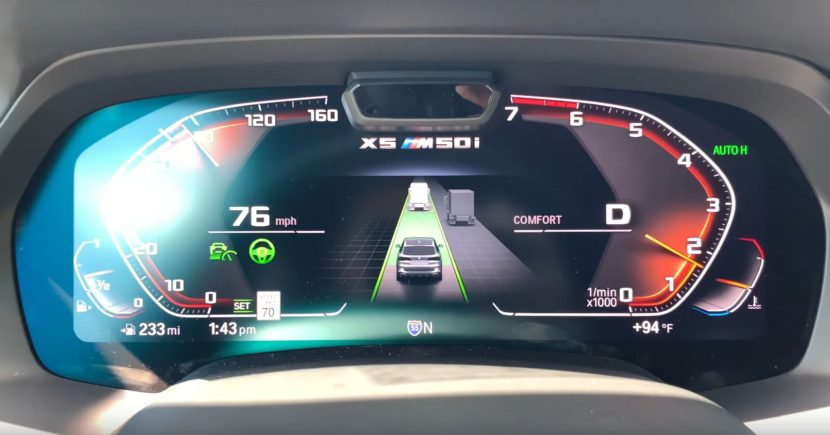
\includegraphics[width=0.6\textwidth]{Figures/bmw.jpg}
	\caption{BMW driving assistent - umiestnenie kamery na snímanie vodiča.\cite{bmw2019assistent}}
	\label{fig:bmwAssistent}
\end{figure}

 Táto diplomová práca je však zameraná aj na detekciu celého tela vodiča a nielen jeho tváre. 







\newpage
\section{Využitie sférických kamier na detekciu obrazu}
\label{sec:Spherical cameras}

Výstup z kamery je reprezentovaný 2D snímkou, ktorá však zachytáva obraz z celého svojho okolia. Medzi najznámejšie projekcie na zachytenie 3D obrazu patrí equirectangular panorama projection, ktoré je definované dvomi uhlami: latitude  $ \omega \in [-90^\circ , +90^\circ ]$ a longitude $\lambda \in [-180^\circ , +180^\circ ]. $

\newpage
\subsection{Použitie v analýze videa}
- problem s rozlišenim , skreslenim , formatom atd.. 
- 


\subsection{Technické parametre}
Go PRO:

THETA:

Senzor	FishEye CMOS 2x12MPix
Maximálne rozlíšenie (Video)	4K  30fps
Maximálne rozlíšenie (Fotografia)	14.5MP (5376x2688px)
Svetelnosť	f2.0
Vnútorná pamäť	19GB

\newpage
\section{Program}
\label{sec:Program}
- Popis programu\\
- jazyk Python\\
- pouzite kniznice\\


\newpage
\subsection{Požiadavky a návrh programu}
- poziadavky \\
- Architekruta programu , schemy


\newpage
\subsection{Detekcia vodiča}
- umiestnenie kamery, detekcia vodiča\\
 - vyber TF vs OpenPose



\newpage
\subsubsection{Neurónová sieť}
-NN klasifikator\\
- trenovanie \\
- testovanie



\newpage
\subsection{Orientácia hlavy}
- Haar  priznaky ,\\
- prevod 2D na 3D \\
- smerova priamka

\newpage
\subsection{Výstup programu}
obrazky\\
tabulky

\newpage
\subsection{Porovnanie výsledkov}
porovnanie


\newpage
\subsection{Využitie zozbieraných dát}
pouzitie v buducnosti


\newpage
\subsection{Používateľská príručka}
python program.py --use-openPose=true


\newpage
\section{Možnosti vylepšenia detekcie}
\label{sec:Možnosti vylepšenia detekcie}
Zhrnutie vysledkov


\newpage
\section{Záver}
\label{sec:Zaver}
Zhrnutie vysledkov







\bibliography{literatura}














\end{document}
